\documentclass{beamer}
%
% Choose how your presentation looks.
%
% For more themes, color themes and font themes, see:
% http://deic.uab.es/~iblanes/beamer_gallery/index_by_theme.html
%
\mode<presentation>
{
  \usetheme{Darmstadt}      % or try Darmstadt, Madrid, Warsaw, ...
  \usecolortheme{crane} % or try albatross, beaver, crane, ...
  \usefonttheme{default}  % or try serif, structurebold, ...
  \setbeamertemplate{navigation symbols}{}
  \setbeamertemplate{caption}[numbered]
  \usepackage{tikz}
  \usepackage{pgfplots}
  \usepackage{pgf}
  \usepackage{units}
  \usepackage{metalogo}
  \usepackage{graphicx}
  \usepackage{caption}
  \usepackage{subcaption}
  \usepackage[mode=buildnew]{standalone}% requires -shell-escape
  \usepgfplotslibrary{groupplots}
  \usepackage{amsmath}
} 

\usepackage[english]{babel}
\usepackage[utf8x]{inputenc}
\setbeamertemplate{footline}[frame number]

\title{LAS Thesis project kickoff meeting}
\author{Moritz Wolter}

\date{\today}

\begin{document}
\begin{frame}
  \titlepage
\end{frame}


% Uncomment these lines for an automatically generated outline.
\begin{frame}{Outline}
  \tableofcontents
\end{frame}

\section{Project Overview}
\begin{frame}{Project Overview}
	\begin{itemize}
		\item Transcribe speech utterances to characters. 
		\item Use a listen attend and spell (LAS) model to do this.
		\item Train model components jointly.
	\end{itemize}
\end{frame}

\section{Listen Attend and Spell}

\begin{frame}{The LAS-Architecture}
\begin{figure}
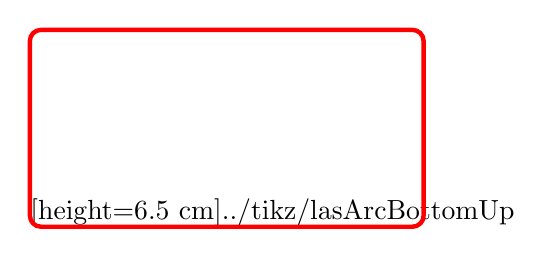
\begin{tikzpicture}
    \node[anchor=south west,inner sep=0] at (0,0) {\includestandalone[height=6.5 cm]{../tikz/lasArcBottomUp}};
    \draw[red,ultra thick,rounded corners] (0.0,0.0) rectangle (5.0,2.5);
\end{tikzpicture}
\caption{The LAS architecture}
\label{fig:las}
\end{figure}
\end{frame}


\begin{frame}{What is Tensorflow?}
	\begin{itemize}
		\item \textquotedblleft TensorFlow is an interface for expressing machine learning algoritms and an implementation for executing such algorithms. \textquotedblright \footnote{TensorFlow:
			  Large-Scale Machine Learning on Heterogeneous Distributed Systems, Abadi et al, Google Research.}
		\item Computations are described by directed graphs. 
		\item Data-Tensors flow along graph edges.
		\item Graphs are constructed using user specified elementary
			  operations.
		\item Computations are started by requesting certain values, which leads
			  to (partial) evaluation of the graph.
	\end{itemize}
\end{frame}


\begin{frame}{Tensorflow}
\begin{figure}
\centering
\includegraphics[width=0.7\linewidth]{../png/net1}
\caption{A simple linear node in tensorboard}
\label{fig:net1}
\end{figure}
\end{frame}

\section{Planning}
\begin{frame}{What happend so far? What will happen next?}
\begin{itemize}
\item What happend so far?
	\begin{enumerate}
		\item Literature overview.
		\item Learned how to use tensorflow.
		\item Looked into timit and aurora4.
	\end{enumerate}
\item What will happen next?
		\begin{enumerate}
			\item Finish implementing a skeleton LAS on Timit. 
			\item Decoding with beam search.
			\item Port to aurora4.
		\end{enumerate}
\end{itemize}
\end{frame}


\section{Questions}
\begin{frame}{Summary and Questions}
	The presentation covered:
	\begin{itemize}
		\item Input feature generation.
		\item The LSTM building block.
		\item A LAS-Architecture overview.
		\item The tensorflow toolbox.
		\item The plan.
	\end{itemize}
	Thank you for your attention. Questions? \\
	\texttt{moritzalexander.wolter@student.kuleuven.be}
\end{frame}


\end{document}
